\documentclass[main-physics.tex]{subfiles}

\begin{document}



\section{Changing Motion}

\subsection{Average Acceleration}

% Recall that \gls{velocity} is the speed and direction of an object. \Gls{acceleration} is the rate of change in velocity. Acceleration is about an object's speeding up, slowing down, or changing direction.

\Gls{acceleration} is the change in velocity divided by a period of time during which the change occurs. The SI units of velocity are meters per second (m/s), and the SI units for time are seconds (s), so the SI units for acceleration are \SI{}{m/s^2}. Acceleration occurs when a car, for example, starts from rest and acquires a speed of \SI{60}{mph} in a brief time of 2.5 seconds. 

\begin{center}
    \begin{tikzpicture}
        \begin{axis}[width=10cm,height=2.5cm,
            xmin=0,xmax=12,
            ymin=0,ymax=12,
            ticks=none,
            axis line style={draw=none}, 
            clip=false,
        ]
            \node at (0,0) {\mycar} node[above=5mm] {$t=0\ ,\ v=0$};
            \draw (10,0) node[left=-3mm] {\textcolor{black!15}{\mycar}}
            node[left=-5mm] {\textcolor{black!30}{\mycar}}
            node {\mycar} node[above=5mm] {$t=\SI{2.5}{s}\ ,\ v=\SI{26.8}{m/s}$};
        \end{axis}
    \end{tikzpicture}
\end{center}

\vspace{1em}

\Gls{average acceleration} is given by

\begin{equation} \label{33EGTg}
    a = \frac{\text{change in velocity}}{\text{change in time}} = \frac{\Delta{v}}{\Delta{t}} = \frac{v_f - v_0}{t_f - t_0}
\end{equation}

\begin{center}
    \begin{tabular}{cl|cl}
    \hline
    \textbf{Symbol} & \textbf{Quantity} & \textbf{SI Base Unit} & \textbf{Unit Symbol}  \\
    \hline\hline
    \rule{0pt}{2.5ex}
        $a$ & average acceleration & meter per second squared & \SI{}{\meter/\second^2}\\
        $\Delta{v}$ & change in velocity & meter per second & m/s\\
        $\Delta{t}$ & elapsed time & second & s \\
    \hline
        $v_f$ & final velocity & meter per second & m/s\\
        $v_0$ & initial velocity & meter per second & m/s\\
        $t_f$ & final time & second & s \\    
        $t_0$ & initial time & second & s \\
        \hline
    \end{tabular}
    \captionsetup{type=figure,margin=1in,font=scriptsize}
    \captionof{figure}{The quantities, symbols, and units involved in the average acceleration equation. Elapsed time is also known as \textit{change in time} or simply \textit{time}, and so $\Delta{t}$ is often just written as $t$.}
\end{center}

Average acceleration is distinguished from \gls{instantaneous acceleration}, which is acceleration at a specific instant in time. The magnitude of acceleration is often not constant over time. For example, runners in a race accelerate at a greater rate in the first second of a race than during the following seconds. You do not need to know all the instantaneous accelerations at all times to calculate average acceleration. All you need to know is the change in velocity (i.e., the final velocity minus the initial velocity) and the change in time (i.e., the final time minus the initial time), as shown in Equation \eqref{33EGTg}. A component of the average acceleration can be positive, negative, or zero. A \gls{negative acceleration} component is simply an acceleration in the negative direction along that axis. When the motion is in one dimension, we often simply refer to this as negative acceleration, and acceleration in the positive direction as positive acceleration.

\vspace{1em}

Keep in mind that although acceleration points in the same direction as the \textit{change} in velocity, it is not always in the direction of the velocity itself. When an object slows down, its acceleration is opposite to the direction of its velocity. In everyday language, this is called deceleration; but in physics, it is acceleration---whose direction happens to be opposite that of the velocity. For now, let us assume that motion to the right along the $x$-axis is positive and motion to the left is negative.

\vspace{1em}

Figure ?.?? shows a car with positive acceleration and one with negative acceleration. The arrows represent vectors showing both direction and magnitude of velocity and acceleration.

\begin{center}
    \begin{tikzpicture}
        \begin{axis}[width=8cm,height=2.5cm,
            xmin=2,xmax=8,
            ymin=0,ymax=12,
            ticks=none,
            axis line style={draw=none}, 
            clip=false,
        ]
            \node at (4,0) {\mycar};
            \draw (6,0) node[left=-3mm] {\textcolor{black!15}{\mycar}}
            node[left=-5mm] {\textcolor{black!30}{\mycar}}
            node {\mycar};
            \draw[->] (3.5,12) -- ++(axis direction cs: 2,0) node[right] {$v$} node[above=2mm,pos=0.5] {Speeding Up};
            \draw[->] (4,8) -- ++(axis direction cs: 1,0) node[right] {$a$};
        \end{axis}
    \end{tikzpicture}%
    \hspace{1cm}
    \begin{tikzpicture}
        \begin{axis}[width=8cm,height=2.5cm,
            xmin=2,xmax=8,
            ymin=0,ymax=12,
            ticks=none,
            axis line style={draw=none}, 
            clip=false,
        ]
            \node at (6,0) {\mycar};
            \draw (4,0) node[left=-3mm] {\textcolor{black!15}{\mycar}}
            node[left=-5mm] {\textcolor{black!30}{\mycar}}
            node {\mycar};
            \draw[->] (3.5,12) -- ++(axis direction cs: 2,0) node[right] {$v$} node[above=2mm,pos=0.5] {Slowing Down};
            \draw[<-] (4,8) -- ++(axis direction cs: 1,0) node[right] {$a$};
        \end{axis}
    \end{tikzpicture}
\end{center}

Velocity and acceleration are both vector quantities. Recall that vectors have both magnitude and direction. An object traveling at a constant speed does accelerate if it changes direction. So, turning the steering wheel of a moving car makes the car accelerate because the velocity changes direction.

\begin{example} \label{KVt2BG}
   Charlie's Porsche 911, a fancy car, goes from \SI{45}{m/s} to \SI{67}{m/s} (\SI{101}{mph} to \SI{150}{mph}) in \SI{4.3}{s}. What is his car's average acceleration? 
\end{example}

\Solution We are given the initial and final velocities and the elapsed time: $v_0 = \SI{45}{m/s}$, $v_f = \SI{67}{m/s}$, and $\Delta{t} = \SI{4.3}{s}$. The unknown is average acceleration: $a =\ ?$

\vspace{1em}

The given and unknown quantities are related by Equation \eqref{33EGTg} as

\begin{equation*}
    a = \frac{\Delta{v}}{\Delta{t}}
\end{equation*}

where the car's change in velocity is final velocity minus initial velocity:

\begin{equation*}
    \Delta{v} = v_f - v_0 = 67 - 45 = \SI{22}{m/s}
\end{equation*}

Therefore, the average acceleration is

 \begin{equation*}
    a = \frac{\Delta{v}}{\Delta{t}} = \frac{22}{4.3} = \SI{5.1}{m/s^2}
\end{equation*}

This means that the car's velocity increases by 5.1 meters per second with every second that passes.

\endsolution


\begin{example} \label{DcGEnk}
    Charlie drives his Porsche 911 at a constant velocity of \SI{45}{m/s} (\SI{101}{mph}) for 10 seconds. What is the average acceleration of the car?
\end{example}

\Solution We are given initial velocity and elapsed time: $v_0 = \SI{45}{m/s}$ and $\Delta{t} = \SI{10}{s}$. The unknown is average velocity, which is given by (Eq.~\ref{33EGTg})

\begin{equation*}
    a = \frac{\Delta{v}}{\Delta{t}} = \frac{v_f - v_0}{\Delta{t}}
\end{equation*}

The difference between this example and Example \ref{KVt2BG} is that here ``constant velocity'' means there's no change in velocity: 

\begin{equation*}
    \Delta{v} = \text{change in velocity} = \SI{0.0}{m/s}
\end{equation*}

Therefore,

\begin{equation*}
    a = \frac{\Delta{v}}{\Delta{t}} = \frac{0.0}{10.0} = \SI{0.0}{m/s^2}
\end{equation*}

An acceleration of zero means the car does not speed up nor slow down, which is exactly what we expect for a car moving at constant velocity.

\endsolution


\begin{example}
    A golf ball rolls at \SI{2.7}{m/s} near the top of an inclined ramp. When it starts rolling down the ramp, it accelerates at \SI{4.9}{m/s^2} for \SI{5.0}{s}. What is the golf ball's final velocity?
\end{example}

\Solution We are given the ball's initial velocity, acceleration, and time:

\begin{equation*}
    v_0 = \SI{2.7}{m/s}, \quad
    a = \SI{4.9}{m/s^2}, \quad
    \Delta{t} = \SI{5.0}{s}
\end{equation*}

We want to find the final velocity: $v_f =\ ?$. These quantities are related by Equation \ref{KVt2BG} for average acceleration:

\begin{equation*}
    a = \frac{v_f - v_0}{\Delta{t}}
\end{equation*}

Substituting given values leads to

\begin{equation*}
    4.9 = \frac{v_f - 2.7}{5.0}\ ,
\end{equation*}

We solve this equation for final velocity ($v_f$) as follows:

\begin{align*}
    \textbf{Put $v_f$ on left} \qquad & \frac{v_f - 2.7}{5.0} = 4.9\\[1ex]
    \textbf{Multiply by 5.0} \qquad & \frac{v_f - 2.7}{\cancel{5.0}} \mathbin{\color{red}\times} \textcolor{red}{\cancel{5.0}} = 4.9 \mathbin{\color{red}\times} \textcolor{red}{5.0}\\[1ex] 
    \textbf{Simplify} \qquad & v_f - 2.7 = 24.5\\[1ex]
    \textbf{Add 2.7} \qquad & v_f - 2.7 \mathbin{\color{red} +} \textcolor{red}{2.7} = 24.5 \mathbin{\color{red} +} \textcolor{red}{2.7}\\[1ex]
    \textbf{Simplify} \qquad & v_f = 27.2
\end{align*}

Therefore the final velocity of the golf ball is \SI{27.2}{m/s}.

\endsolution

\begin{example}
  A vehicle accelerates a at \SI{2.47}{m/s^2}. How much time (in seconds) does it take this car to change its speed from \SI{18}{m/s} to \SI{25}{m/s}?  
\end{example}

\Solution We are given acceleration and initial and final velocities:

\begin{equation*}
    a = \SI{2.47}{m/s^2}\ , \quad
    v_0 = \SI{18}{m/s}\ , \quad
    v_f = \SI{25}{m/s}
\end{equation*}

We want to find the elapsed time: $\Delta{t} =\ ?$ These known and unknown quantities are related by Equation \eqref{33EGTg} as

\begin{equation*}
    a = \frac{v_f - v_0}{\Delta t}
\end{equation*}

Substituting known values leads to

\begin{equation*}
    2.47 = \frac{25 - 18}{\Delta t}\ ,
\end{equation*}

or, more simply, to

\begin{equation*}
    2.47 = \frac{7}{\Delta t}
\end{equation*}

We solve this equation for elapsed time ($\Delta t$) as follows:

\begin{align*}
    \hspace{-10em} \textbf{Multiply by $\Delta t$} \hspace{5em} & 2.47 \cdot \textcolor{red}{\Delta t} =  \frac{7}{\cancel{\Delta t}} \cdot \textcolor{red}{\cancel{\Delta t}}\\[1ex]
    \hspace{-10em} \textbf{Simplify} \hspace{5em} & 2.47 \cdot \Delta t = 7\\[1ex]
    \hspace{-10em} \textbf{Divide by 2.47} \hspace{5em} & \frac{\cancel{2.47} \cdot \Delta t}{\textcolor{red}{\cancel{2.47}}} = \frac{7}{\textcolor{red}{2.47}}\\[1ex]
    \hspace{-10em} \textbf{Simplify} \hspace{5em} & \Delta{t} = 2.83
\end{align*}

Therefore, it takes this vehicle 2.83 seconds to undergo the given change in velocity.

\endsolution


\subsection{Velocity vs.~Time Graphs}

Recall that velocity is the rate of change of displacement, and acceleration is the rate of change of velocity. As we saw previously, a velocity vs.~time graph plots velocity on the vertical axis and time on the horizontal. The velocity curve tells us whether an object is speeding up, slowing down, or traveling with a constant velocity (i.e., speed).


\begin{example} \label{AbDF59}
    Lance, the bicyclist, starts from rest on a bicycle and acquires a greater speed over time. The graph below represents his motion. What is his average acceleration?
\end{example}


\begin{center}
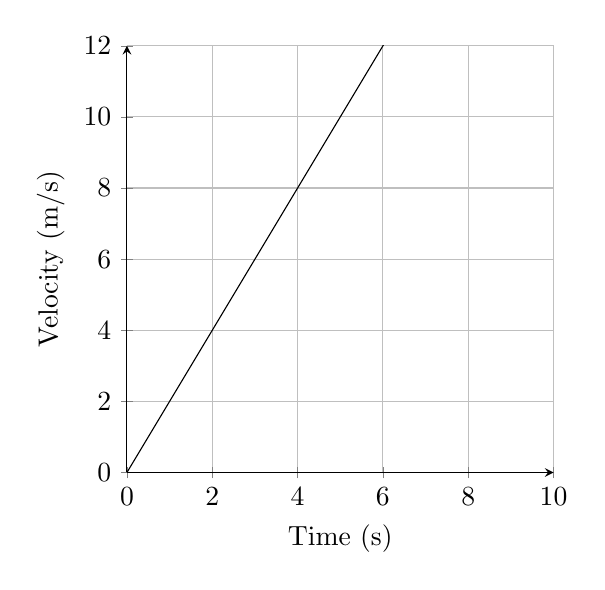
\begin{tikzpicture}
\begin{axis}[width=7cm, height=7cm,
        axis lines=left,
        ymin=0, ymax=12,
        xmin=0, xmax=10,
        ylabel = Velocity (m/s),
        xlabel = Time (s),
        grid=both,
    ]
    \draw plot[domain=0:20,samples=3] (\x,{2*\x});
\end{axis}
\end{tikzpicture}  
\end{center}

\Solution The graph contains plenty of velocity and time information. Since the plot is a straight line, we can select \textit{any} two points on the line to calculate average acceleration. 

\vspace{1em}

Let's define initial and final times as 2 and 6 seconds, respectively. This, consequently, defines initial and final velocities as 4 and 12 meters per second, according to the graph.

\begin{center}
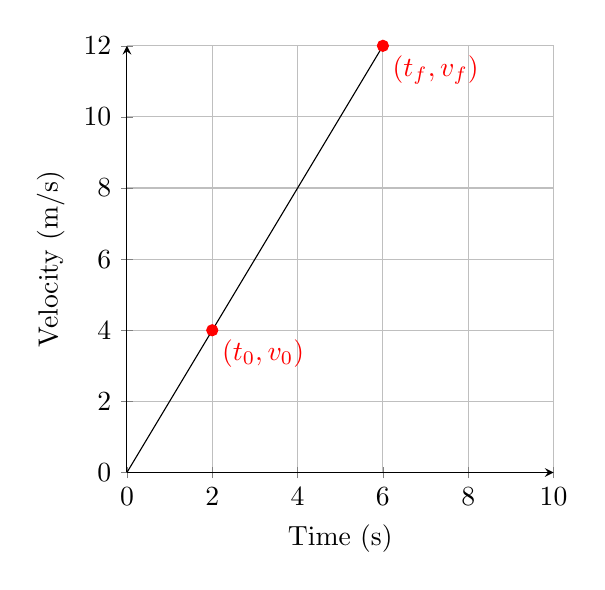
\begin{tikzpicture}
\begin{axis}[width=7cm, height=7cm,
        axis lines=left,
        ymin=0, ymax=12,
        xmin=0, xmax=10,
        ylabel = Velocity (m/s),
        xlabel = Time (s),
        grid=both,
        clip=false,
    ]
    \draw plot[domain=0:6,samples=3] (\x,{2*\x});
    \draw[red,fill=red] (2,4) circle (2pt) node[below right] {$(t_0,v_0)$};
    \draw[red,fill=red] (6,12) circle (2pt) node[below right] {$(t_f,v_f)$};
\end{axis}
\end{tikzpicture}  
\end{center}

So, from the graph, we are given

\begin{equation*}
    t_0 = \SI{2}{s}\ ,\ t_f = \SI{6}{s}\ ,\ 
    v_0 = \SI{4}{m/s}\ ,\ v_f = \SI{12}{m/s}\ ,
\end{equation*}

keeping in mind that we could have selected any two points on the line. The unknown is average acceleration: $a =\ ?$ The given and unknown quantities are related by Equation \eqref{33EGTg} as

\begin{equation*}
    a = \frac{\Delta{v}}{\Delta{t}} = \frac{v_f - v_0}{t_f - t_0}
\end{equation*}

Substituting known values leads to

\begin{equation*}
    a = \frac{12 - 4}{6 - 2} = \SI{2}{m/s^2}
\end{equation*}

Lance's acceleration is 2 meters per second squared. That is, his speed increases at a rate of \SI{2}{m/s} every second.

\endsolution

\begin{example}
    Using a slingshot, Bart aims a rock towards the sky and launches it off the edge of a cliff. The rock's motion is represented in the graph below. Calculate the rock's acceleration.
\end{example}

\begin{center}
    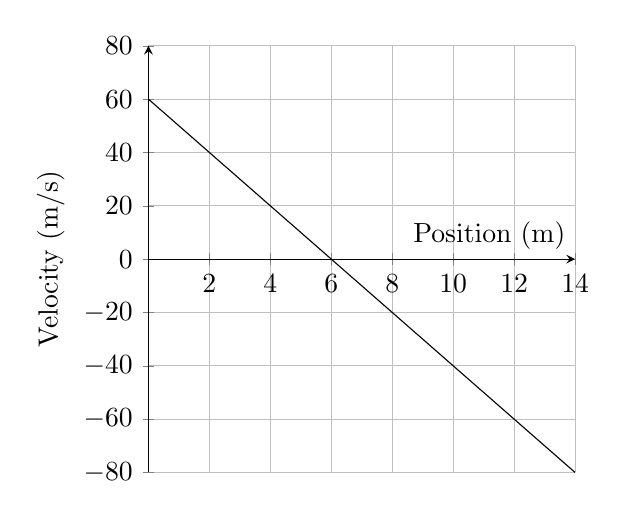
\begin{tikzpicture}
        \begin{axis}[width=7cm,
            height=7cm,
            axis y line=left,
            axis x line=center,
            ylabel={Velocity (m/s)},
            xlabel={Position (m)},
            xmin=0,xmax=14,
            ymin=-80,ymax=80,
            clip=false,
            grid=both,
            xtick={2,4,...,14},
            ytick={-80,-60,...,80}
        ]
        \draw plot[domain=0:14,samples=3] (\x,{-10*\x + 60});
        \end{axis}
    \end{tikzpicture}
\end{center}

\Solution Just as in Example \ref{AbDF59}, we can select any two points on the line to calculate average acceleration. Let's use 0 and 10 seconds as our initial and final times, respectively. Then the initial and final times and initial and final velocities are

\begin{equation*}
    t_0 = 0\ , \quad t_f = \SI{10}{s}\ , \quad
    v_0 = \SI{60}{m/s}\ , \quad v_f = -\SI{40}{m/s}
\end{equation*}

The unknown is average acceleration: $a =\ ?$. By Equation \eqref{33EGTg}, acceleration is

\begin{equation*}
    a = \frac{v_f - v_0}{t_f - t0} = \frac{-40-60}{10-0} = \SI{-10}{m/s^2}
\end{equation*}

Therefore, the rock accelerates at a rate of $-10$ meters per second squared. During the first 6 seconds of motion, the rock moved upwards but always maintained a negative acceleration. Over time, the speed of the rock continued to increase in the negative direction---its velocity became more negative. 

\endsolution

\begin{mdframed}[backgroundcolor=black!10]
    \centering
    \textbf{In a velocity vs.~time graph, displacement is the area under the curve.}
\end{mdframed}


\begin{example}
The velocity-time graph shows the motion of an accelerating object. What is the object's displacement throughout the entire time interval?
\end{example}

\begin{center}
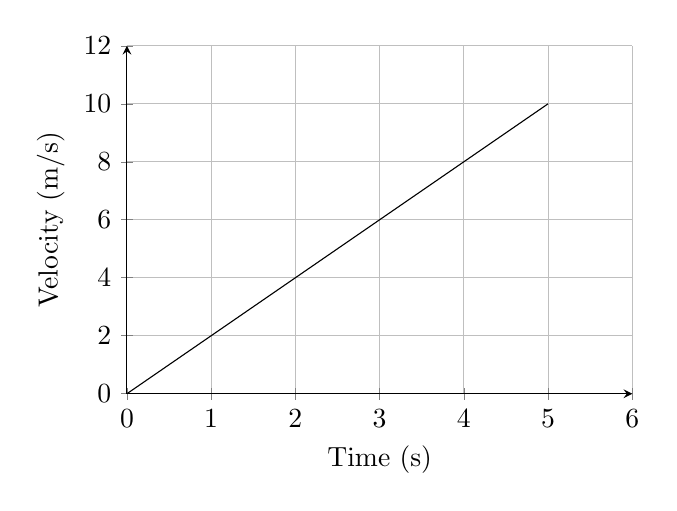
\begin{tikzpicture}
\begin{axis}[width=8cm, height=6cm,
        axis lines=left,
        ymin=0, ymax=12,
        xmin=0, xmax=6,
        ylabel = Velocity (m/s),
        xlabel = Time (s),
        grid=both,
        ytick={0,2,...,12}
    ]
    \draw plot[domain=0:5,samples=3] (\x,{2*\x});
\end{axis}
\end{tikzpicture}
\end{center}

\Solution Displacement is the area under the curve in a velocity vs.~time graph. The bounded area is a right triangle, whose area is given by its base ($b$) multiplied by its height ($h$), divided by 2:

\begin{equation} \label{5kz27x}
    A = \frac{b h}{2} 
\end{equation}

\begin{center}
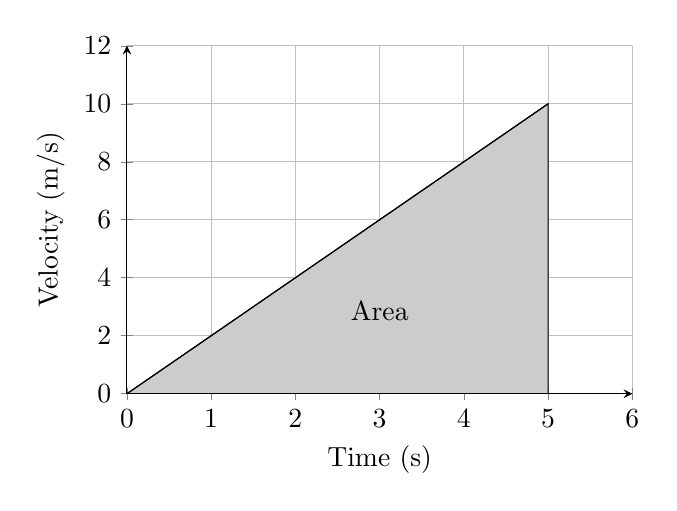
\begin{tikzpicture}
\begin{axis}[width=8cm, height=6cm,
        axis lines=left,
        ymin=0, ymax=12,
        xmin=0, xmax=6,
        ylabel = Velocity (m/s),
        xlabel = Time (s),
        grid=both,
        ytick={0,2,...,12}
    ]
    \draw[fill=black!20] (0,0) -- (5,10) -- (5,0) -- (0,0) node[pos=0.4,above=8mm] {Area};
    \draw plot[domain=0:5,samples=3] (\x,{2*\x});
\end{axis}
\end{tikzpicture}
\end{center}

The base is 5, the height is 10, so the triangle's area is

\begin{equation*}
    A = \frac{bh}{2} = \frac{5 \times 10}{2} = 25
\end{equation*}

Therefore, the object's displacement is \SI{25}{m}.

\begin{example} \label{BksbmH}
    A person on a hoverboard drives to the left, slows down, comes to a stop, turns around, and drives to the right at an increasing speed. Their motion is represented by the graph below. Calculate their displacement throughout the time interval.
\end{example}

\begin{center}
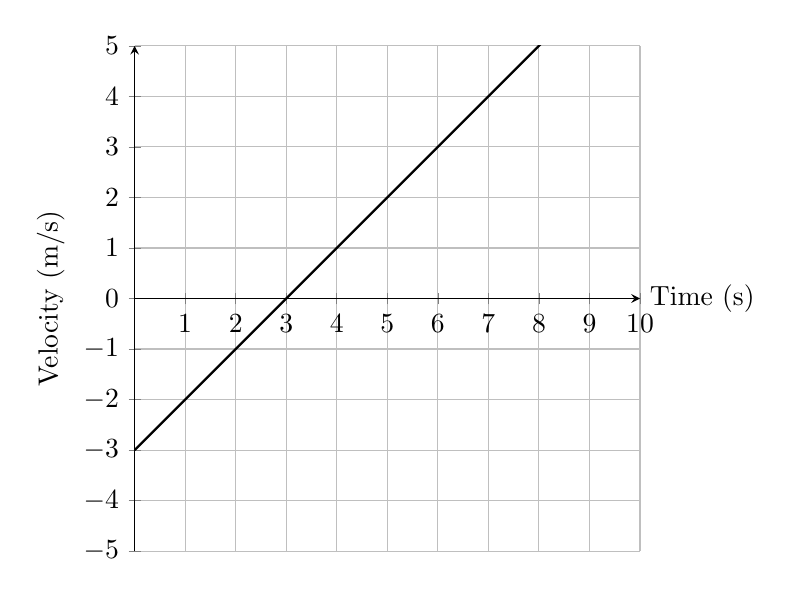
\begin{tikzpicture}
\begin{axis}[axis y line=left, 
        axis x line=center,
        width=8cm,height=8cm,
        ymin=-5, ymax=5,
        xmin=0, xmax=10,
        ylabel = Velocity (m/s),
        xlabel = Time (s),
        grid=both,
        ytick={-5,-4,...,5},
        xtick={0,1,...,10},
        every axis x label/.style={at={(current axis.right of origin)},anchor=west},
    ]
\addplot[mark=none,thick,domain=0:10,]
    {-3 + x};
\end{axis}
\end{tikzpicture}
\end{center}

\Solution You should revisit Example \ref{HjmJqM}, as its solution is similar to this one. Here we see that there are two areas bounded by the curve. Area $A_1$ is negative, representing a negative displacement, because it is below the horizontal axis.  

\begin{center}
    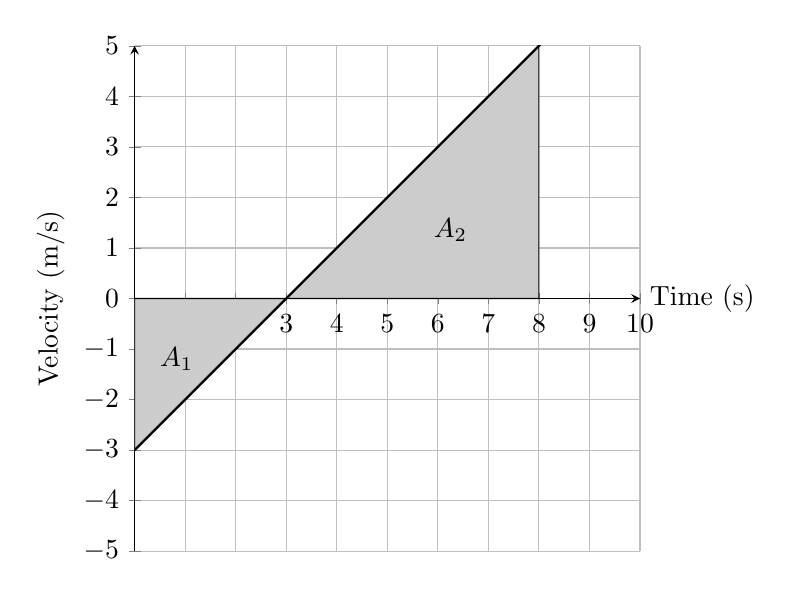
\begin{tikzpicture}
        \begin{axis}[axis y line=left, 
                axis x line=center,
                width=8cm,height=8cm,
                ymin=-5, ymax=5,
                xmin=0, xmax=10,
                ylabel = Velocity (m/s),
                xlabel = Time (s),
                grid=both,
                ytick={-5,-4,...,5},
                xtick={0,1,...,10},
                every axis x label/.style={at={(current axis.right of origin)},anchor=west},
            ]
        \draw[fill=black!20] (0,0) -- (3,0) -- (0,-3) -- (0,0) node[pos=0.6,right=2mm] {$A_1$};
        \draw[fill=black!20] (3,0) -- (8,5) -- (8,0) -- (3,0) node[pos=0.35,above=6mm] {$A_2$};
        \addplot[mark=none,thick,domain=0:10,]
            {-3 + x};
        \end{axis}
    \end{tikzpicture}
\end{center}

By Equation \eqref{5kz27x}, the area of a right triangle is half of the product of base and height:

\begin{equation*}
    A = \frac{bh}{2}
\end{equation*}

$A_1$ has a base of 3 and height of $-3$, so its area is

\begin{equation*}
    A_1 = \frac{(3)(-3)}{2} = -4.5
\end{equation*}

Area $A_2$ has a base of 5, as it encompasses a time interval from 3 to 8 seconds, and a height of 5, so its area is

\begin{equation*}
    A_2 = \frac{(5)(5)}{2} = +12.5
\end{equation*}

The total area is the sum of smaller areas:

\begin{equation*}
    A = A_1 + A_2 = -4.5 + 12.5 = 8.0
\end{equation*}

Therefore, the person's displacement is $+\SI{8.0}{m}$, or 8 meters to the right.

\endsolution





\cyanhrule

\subsection{Exercises}

\begin{exercise} \label{eBsToU}
    Alan's Porsche 911 goes from 0 to \SI{60}{mph} (\SI{26.8}{m/s}) in \SI{2.5}{s}. What is the car's average acceleration? 
\end{exercise}


\begin{exercise} \label{kVZPeG}
  Moby starts at rest and skates down a ramp to a velocity of \SI{15}{m/s} in 5.0 seconds. What is Moby's average acceleration? 
\end{exercise}

\begin{exercise} \label{Vth5N8}
    A subway train accelerates from rest to \SI{8.33}{m/s} in \SI{20.0}{s}. What is the average acceleration during that time interval?
\end{exercise}

\begin{exercise}
    The same train departs from the station from rest and accelerates at \SI{0.753}{m/s^2}. Complete the table below, calculating changes in the train's velocity across time.

\begin{center}
    \begin{tabular}{c|l}
        \textbf{Time (s)} & \textbf{Velocity (m/s)} \\
        \hline
        0 & 0.000\\
        1 & $0.000 + {\color{red}0.753}$\\
        2 & $0.753 + {\color{red}0.753} = 1.506$ \\
        3 & $1.506 + {\color{red}0.753} = 2.259$ \\
        4 & $2.259 + {\color{red}0.753} = 3.012$ \\
        \vdots &  \\
        17 &  \\
    \end{tabular}
\end{center}
\end{exercise}


\begin{exercise} \label{XSJU8b}
    Charles drives a car and accelerates from rest to \SI{12.8}{m/s} in \SI{17.0}{s}. What is the average acceleration during that time interval?
\end{exercise}

\begin{exercise} \label{57fIMa}
An object travels in one direction at a constant velocity, then instantaneously changes direction to a slower speed. Calculate the object's displacement throughout the entire time interval.
\end{exercise}

\begin{center}
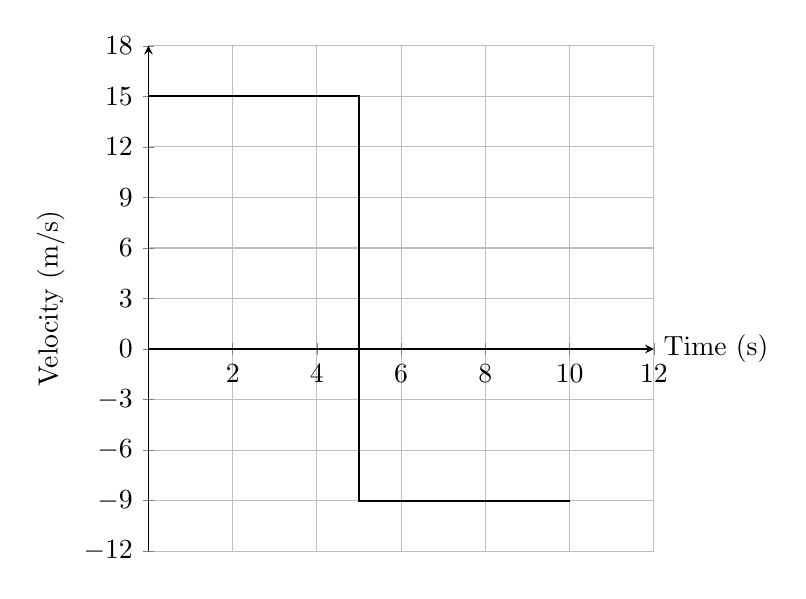
\begin{tikzpicture}
\begin{axis}[width=8cm,height=8cm,
    axis y line=left, 
    axis x line=center,
    xlabel = Time (s),
    ylabel = Velocity (m/s),
    ymin=-12, ymax=18,
    xmin=0, xmax=12,
    ytick={-12,-9,...,18},
    xtick={0,2,...,12},
    grid=both,
    x label style={anchor=west},
    clip=false,
]

    \draw[thick] (0,15) -- (5,15) -- (5,-9) -- (10,-9);
\end{axis}
\end{tikzpicture}
\end{center}

\begin{exercise} \label{kARt6e}
The graph represents an object's motion. What is the displacement of the object throughout the entire time interval?
\end{exercise}

\begin{center}
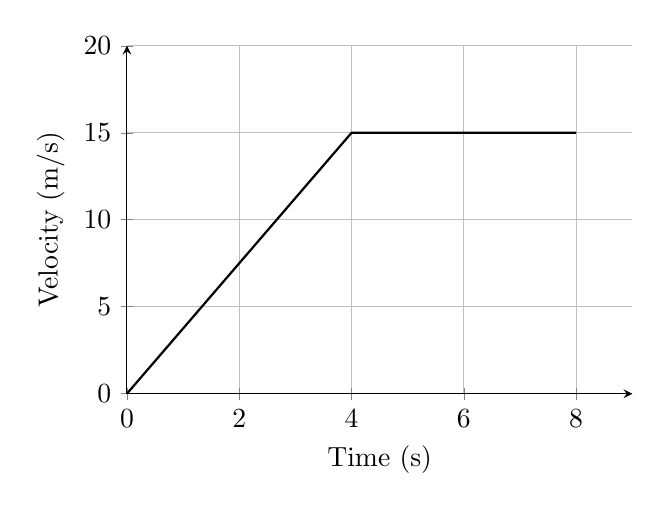
\begin{tikzpicture}
\begin{axis}[width=8cm, height=6cm,
        axis lines=left,
        ymin=0, ymax=20,
        xmin=0, xmax=9,
        ylabel = Velocity (m/s),
        xlabel = Time (s),
        grid=both,
        ytick={0,5,...,20},
    ]
    \draw[thick] (0,0) -- (4,15) -- (8,15);
\end{axis}
\end{tikzpicture}
\end{center}


\subsection{Answers to Select Exercises}
\ref{eBsToU}. \SI{10.7}{m/s^2}\\
\ref{kVZPeG}. \SI{3.0}{m/s^2}\\
\ref{Vth5N8}. \SI{0.417}{m/s^2}\\
\ref{XSJU8b}. \SI{0.753}{m/s^2}\\
\ref{57fIMa}. \SI{30}{m}\\
\ref{kARt6e}. \SI{90}{m}\\





\end{document}


\begin{enumerate}
\setlength\itemsep{0.1ex}
    \item \label{goal:Calc_DeltaV} Calculate change in velocity given initial and final velocities
    \item Calculate acceleration of an object starting from rest given final velocity and time
    \item Calculate acceleration given initial velocity, final velocity, and time
    \item \label{goal:Solve_AccelEq_FinalVel}  Use the $a = \Delta{v}/\Delta{t}$ equation to solve for final velocity given initial velocity, acceleration, and time
    \item \label{goal:Solve_AccelEq_Time} Use the $a = \Delta{v}/\Delta{t}$ equation to solve for time given initial velocity, final velocity, and acceleration.
    \item Understand the relation between displacement and area bounded by a curve in a velocity vs.~time graph
    \item Calculate displacement in a velocity vs.~time graph for a region of constant velocity.
    \item Calculate displacement in a velocity vs.~time graph for a region of constant acceleration.
\end{enumerate}